% include the figures path relative to the master file
\graphicspath{ {./content/intro/figures/} }

\section{Introduction}
\label{sec:descr}  % \label{} allows reference to this section
Malignant melanoma is a type of skin cancer and although it accounts for almost 2\% of all skin cancer cases, it is the deadliest type causing the vast majority of deaths. 
The incidence of melanoma has increased in the past decades to currently reach 132,000 melanoma cases, according to the World Health Organisation~\cite{WoH}.
The \Ac{acs} also reported the estimated deaths of melanoma in 2014 as $9710$ individuals and new cases as $76,100$ individuals~\cite{CancerFactsFigures2014}. 
%At the same time, however, the patient survival rate significantly has increased, thanks to early diagnosis and treatment of melanoma.
Melanoma cancer is incurable in its advanced stages and the patient should go through surgery, possibly immunotherapy, chemotherapy, and/or radiation therapy. 
However, if it is diagnosed at its early stage, it is the most treatable kind of cancer~\cite{CancerFactsFigures2014,forsea2012melanoma}.
In fact the patient survival rate has increased significantly, in the past decades, thanks to early diagnosis and treatment of melanoma in its early stages. 

\begin{figure*}
\begin{center}
  \hspace*{\fill}
  \subfloat[Melanoma lesion]{
    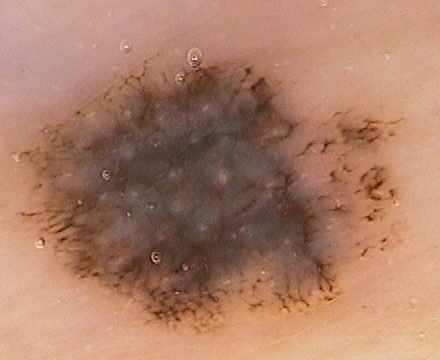
\includegraphics[width=0.2\textwidth, height= 0.12\textheight]{M1_PH2.png}}\hfill
  \subfloat[Dysplastic lesion]{
    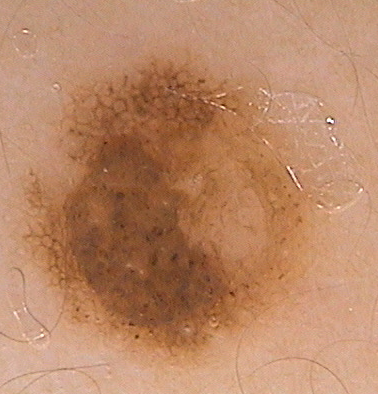
\includegraphics[width=0.2\textwidth, height= 0.12\textheight]{D1_PH2.png}}\hfill
  \subfloat[Benign lesion]{
    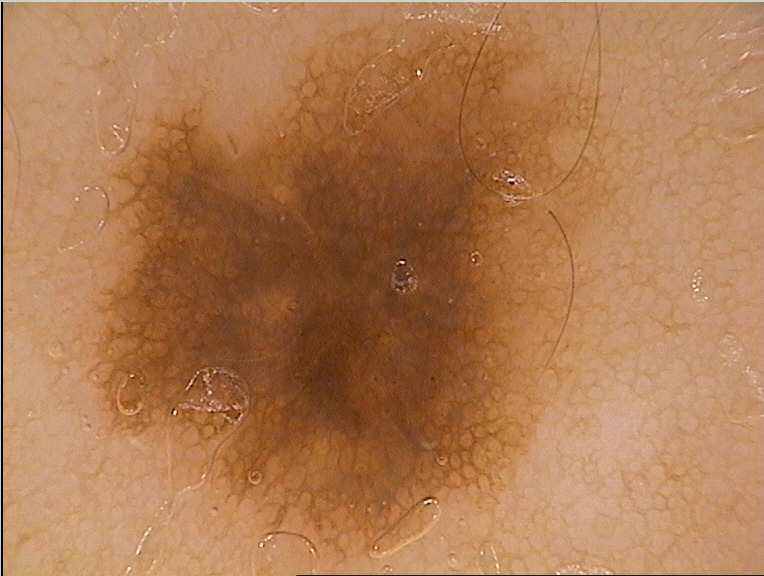
\includegraphics[width=0.2\textwidth, height= 0.12\textheight]{B1_PH2.png}}
  \hspace*{\fill}
  \caption{Samples of $PH^2$ dataset, representing melanoma, dysplastic and benign lesions, respectively.}
  \label{fig:PH2samples}
\end{center}
\end{figure*}

{\color{red}Add the ABCDE lexicon here}

The clinical prognosis of early stage of melanoma is based on the ``ABCDE'' rule~\cite{abbasi2004early}, standing for: Asymmetry, irregular Borders, variegated Colors, Diameter greater than \SI{6}{\milli \meter} and Evolving stages of the lesion over time.
At each clinical routine, these criterion are used to visually inspect skin lesions which are acquired through different imaging techniques such as dermoscopy.
The similarity between the lesions and the necessity to perform patients follow-up over years makes visual inspection difficult and more prone to errors.
Thus, \ac{cad} systems based on machine learning and image processing techniques have been proposed to assist the dermatologists and clinicians. 
The proposed algorithms generally attend to mimic the characteristics of the ``ABCDE'' rule and consist of common steps of pre-processing, segmentation and classification of extracted features~\cite{rastgoo2015automatic}.
This sequential architecture is complex and each process of the framework is data-driven. 

In this paper, we propose a more general framework which does not need pre-processing and segmentation of the lesions and is based on sparse coded features and \ac{rf} classifier~\cite{breiman2001random} to detect melanoma in dermoscopic images. 

The rest of this paper is organized as follows: an overview of related work is presented in Sect.\,\ref{sec:rw}.
The proposed method is discuss in Sect.\,\ref{sec:method} while the experiment and obtained results are presented in Sect.\,\ref{sec:exp} and\,\ref{sec:res}, respectively.
Finally the paper is concluded in Sect.\,\ref{sec:con}.



% Some stuff that emac's colegues use
%%% Local Variables:
%%% mode: late
%%% TeX-master: "../../master.tex"
%%% End: \section{introduction}

